% Copyright (C) 2007 Technical University of Liberec.  All rights reserved.
%
% Please make a following refer to Flow123d on your project site if you use the program for any purpose,
% especially for academic research:
% Flow123d, Research Centre: Advanced Remedial Technologies, Technical University of Liberec, Czech Republic
%
% This program is free software; you can redistribute it and/or modify it under the terms
% of the GNU General Public License version 3 as published by the Free Software Foundation.
%
% This program is distributed in the hope that it will be useful, but WITHOUT ANY WARRANTY;
% without even the implied warranty of MERCHANTABILITY or FITNESS FOR A PARTICULAR PURPOSE.
% See the GNU General Public License for more details.
%
% You should have received a copy of the GNU General Public License along with this program; if not,
% write to the Free Software Foundation, Inc., 59 Temple Place - Suite 330, Boston, MA 021110-1307, USA.
%
%
%
% use PDFLatex to compile this
%

\documentclass[12pt,a4paper]{report}

%%% remove comment delimiter ('%') and specify encoding parameter if required,
%%% see TeX documentation for additional info (cp1252-Western,cp1251-Cyrillic)
%\usepackage[cp1252]{inputenc}

%%% remove comment delimiter ('%') and select language if required
%\usepackage[english,spanish]{babel}
%\usepackage{czech}
\usepackage{amssymb}
\usepackage{amsmath}
\usepackage{array}
\usepackage{longtable}
\usepackage{tabularx}
\usepackage{graphicx} %[dvips]

\usepackage{fancyvrb}	% extended verbatim environments (for examples of IO files)
\usepackage{hyperref}   % hypertext capabilities, should by last package

\hypersetup{backref,colorlinks=true}  %setup hyperef package

\newcommand{\vari}[1]{{\it #1}}
\newcommand{\ditem}[2]{\item[\vari{#1} {\tt #2}]}
\newenvironment{fileformat}{\tt\begin{flushleft}}{\end{flushleft}}
%
%% ini table environment
\newcommand{\key}[1]{{\tt #1 }}
\newcommand{\type}[1]{{\bf #1}}
%
\newenvironment{initable}[1]{%
        \vspace{4ex}
        \noindent
        Section: \textbf{[#1]}\\
        \begingroup
        %%
        %% internal commands of initable environment
        %%
       \newcommand{\br}{\hfill\break}
        %%
        \renewcommand{\arraystretch}{1.4}
        \renewcommand{\tabcolsep}{2mm}
        \small
        \baselineskip 3ex
        %\begin{longtable}{@{}lp{5cm}p{5cm}p{9cm}}%
        \tabularx{\textwidth}{l>{\centering}p{2cm}>{\raggedright}p{2cm}>{\raggedright\arraybackslash}X}%
        %\renewcommand{\\}{\\[3ex]}%
        \hline\hline
        KEY & TYPE & DEFAULT & DESCRIPTION \\%\endhead
        \hline\hline
}{%
        %\end{longtable}
        \endtabularx
        \endgroup
}

%% ini_table members

%%% remove comment delimiter ('%') and specify parameters if required
%\usepackage[dvips]{graphics}

%%%%%%%%%%%%%%%%%%%%%%%%%%%%%%%%%%%%%%%%%%%%%%%%%%%%%%%%%%%%%%%%%%%%%%%%%%%%%%%%%%%%%%%%%%%%% BEGIN DOCUMENT
%% set specific page layout
\addtolength{\textwidth}{2cm}
\addtolength{\hoffset}{-1.5cm}
\addtolength{\textheight}{4cm}
\addtolength{\voffset}{-2.5cm}
\begin{document}

%%% remove comment delimiter ('%') and select language if required
%\selectlanguage{spanish} 
\thispagestyle{empty}
\begin{center}
\noindent 
\textbf{\LARGE{
  Technical university of Liberec
}}

\vspace{2ex}
\textbf{\LARGE{
  Faculty of mechatronics, informatics\\
  and interdisciplinary studies
}}

\vspace{160pt}

\textbf{\Huge{
FLOW123D
}}

\vspace{1cm}
\textbf{\Large{
version 1.6.6
}}

\vspace{1cm}

\textbf{\Large{
Documentation of file formats \\
and brief user manual.
}}


\vspace{7cm}

\noindent \textbf{\Large{Liberec, 2011}}

\vspace{1cm}

{\bf Acknowledgement.} This work was realized under the state  subsidy of the Czech Republic within the research and development 
project ``Advanced Remediation Technologies and Processes Center'' 1M0554 
-- Program of Research Centers PP2-D01 supported by Ministry of Education.
\end{center}
\noindent 

\noindent

\tableofcontents
\pagebreak
%\setcounter{page}{2}

\parindent=0pt
\parskip=1ex

\chapter{Overview}

Flow123D is a software for simulation of water flow and reactionary solute transport in a heterogeneous 
porous and fractured medium. In particular it is suited for simulation of underground processes in a granite rock massive.
The program is able to describe explicitly processes in 3D medium, 2D fractures, and 1D chanels and exchange between 
domains of different dimension. The computational mesh is therefore collection of 3D tetrahedrons, 2D triangles and 1D line segments.

The water flow model assumes a saturated medium described by Darcy law. For discretization, we use lumped mixed-hybrid finite element method.
We support both steady and unsteady water flow.

The solute transport model can deal with several dissolved substances. It contains non-equilibrium dual porosity model, 
i.e. exchange between mobile and immobile 
pores. There is also model for several types of adsorption in both the mobile and immobile zone. The implemented adsorption models are
linear adsorption, Freundlich isotherm and Langmuir isotherm. The solute transport model uses finite volume discretization 
with up-winding in space and explicit Euler discretization in time. The dual porosity and the adsorption are introduced into transport by operator splitting.
The dual porosity model use analytic solution and the non-linear adsorption is solved numerically by the Newton method.

Reaction between transported substances can be modeled either by a SEMCHEM module, which is slow, but can describe all sorts of reactions. On the other hand,
for reactions of the first order, i.e. linear reactions or decays, we provide our own solver which is much faster. Reactions are coupled with transport 
by the operator splitting method,

The program provides output of the pressure, the velocity and the concentration fields in two file formats. You can use file format of GMSH mesh generator and post-processor 
or you can use output into widely supported VTK format. In particular we recommend Paraview software for visualization and post-processing of VTK data.

The program is implemented in C/C++ using essentially PETSC library for linear algebra. The water flow as well as the transport simulation and reactions can be computed 
in parallel using MPI environment. 

The program is distributed under GNU GPL v. 3 license and is available on the project web page:
http://dev.nti.tul.cz/trac/flow123d

\section{Basic usage}

\subsection{How to run the simulation.}
On the Linux system the program can be started either directly or through a script \verb'flow123d.sh'. When started directly, e.g. by the command
\begin{verbatim}
  > flow123d -s example.ini
\end{verbatim}
the program requires one argument after switch \verb'-s' which is the name of the principal input file. Full list of possible command line arguments is as follows.

\begin{description}
 \item[-s {\bf\it file}] \hfill\\
 	 Set principal INI input file. All relative paths in the INI file are relative against current directory.
 \item[-S {\bf\it file}] \hfill\\
 	Set principal INI input file. All relative paths in the INI file are relative against directory of the INI file. This is equivalent
to change directory to the directory of the INI file at the start of the program.
 \item[-i {\bf\it path}] \hfill\\
 	When there is string \verb"${INPUT}" %$
  	in the any path in the INI file, it will be replaced by given {\it path}.
 \item[-o {\bf\it path}] \hfill\\
 	Every relative path for any output file will be relative to this {\it path}. 
 \item[-l {\bf\it [file\_name]}] \hfill\\
 	Set base name of log files or turn logging off if no file name is given.

\end{description}

All other parameters will be passed to the PETSC library. An advanced user can influence lot of parameters of linear solver. In order to get list of supported options 
use parameter \verb'-help'.


Alternatively, you can use script \verb'flow123d.sh' to start parallel jobs or limit resources used by the program. This script accepts the same parameters as the program itself
and further following additional parameters:

\begin{description}
  \item[-h] \hfill\\
  	Usage overview.
  \item[-t {\bf\it timeout}] \hfill\\
  	Upper estimate for real runing time of the calculation. Kill calculation after {\it timeout} seconds. 
  	Can also be used by PBS to choose appropriate job queue. 
  \item[-np {\bf\it number of processes}] \hfill\\
  	Specify number of parallel processes for calculation.
  \item[-m {\bf\it memory limit}] \hfill\\
  	Limits total available memory to {\it memory limit} bytes.
  \item[-n {\bf\it priority}] \hfill\\
  	Change (lower) priority for the calculation. See {\tt nice} command.
  \item[-r {\bf\it out file}] \hfill\\
  	Stdout and stderr will be redirected to {\it out file}.
\end{description}

On the Windows system we use Cygwin libraries in other to emulate Linux API. Therefore you have to keep the Cygwin libraries within the same direcotry as the program executable.
The Windows package that can be downloaded from project web page contains both the Cygwin libraries and the mpiexec command for starting parallel jobs on the Windows workstations.

Then you can start the sequential run by the command:
\begin{verbatim}
  > flow123d.exe -s example.ini
\end{verbatim}
or the parallel run by the command:
\begin{verbatim}
  > mpiexec.exe -np 2 flow123d.exe -s example.ini
\end{verbatim}
The program accepts the same parameters as the Linux version, but there is no script similar to \verb'flow123d.sh' for the Windows system.


\subsection{Structure of input}

The principal input file of the program is an INI file which contains names of other necessary input files.
Those are the file with calculation mesh (\verb'*.msh'), the file with specification of adjacency between dimensions (\verb'*.ngh'),
the file with material description (\verb'*.mtr') and the file with boundary conditions for the water flow problem (\verb'*.bcd').
For unsteady water flow you have to specify file with initial condition for the pressure (key \verb'Input/Initial') and optionally one can introduce 
file with water sources (key \verb'Input/Sources').

In the case of transport simulation one have to specify also the file with transport boundary conditions (\verb'*.tbc') 
and the file with transport initial condition
for individual substances (\verb'*.tic').

 \begin{figure}[h]
    \begin{center}
      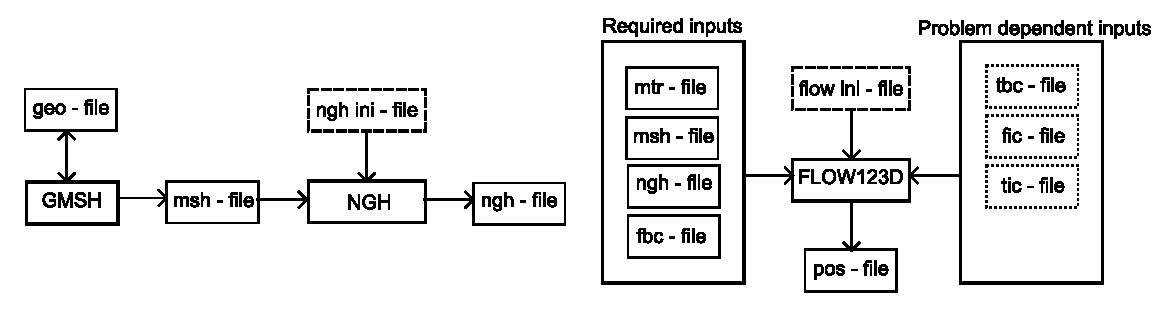
\includegraphics[scale=0.7]{schema.pdf} % 
      \caption{Preparation of input files.}
      \label{obr3}
    \end{center}
  \end{figure}


For the preparation of input files we use several utilities (see Figure \ref{obr3}). 
We usually begin with a \verb'*.geo' file as a description of the domain geometry. This come as an input for the GMSH mesh generator, which produce 
the mesh file. Then we run program \verb'ngh' to produce adjacency file. Finally we can use program \verb'bcd' for the preparation of files with
boundary and initial conditions. The file with material properties has to be created manually, preferably by modifying some of the example problems.
The programs \verb'ngh' and \verb'bcd' are distributed together with flow123d with their own limited documentation.

The output files can be either \verb'*.msh' files accepted by the GMSH or one can use VTK format that can be post-processed by Paraview.

In the following chapter, we briefly describe structure of individual input files in particular the main INI file. In the last chapter, we describe
mathematical models and numerical methods used in the Flow123d.


\chapter{File formats}
\section{Flow123D ini file format}

\normalsize
 \section*{Flow123D ini file format}
 \begin{flushleft}
 Flow123D version: 03.10.08
 \vspace{20pt}
 
 Note: All string values have maximal length MAXBUFF - 1 (=1023).
 \vspace{20pt}
 \end{flushleft}
 
\begin{initable}{Global}
 \key{Problem\_type} & \type{int} & NULL &
 Type of solved problem. Currently supported:\break %\br 
 1 = steady saturated flow\break %\br
 3 = variable-density saturated flow
 \\
 \hline
 \key{Description} & \type{string} & {\it undefined} &
 Short description of solved problem - any text.
 \\
 \hline
 \key{Stop\_time} & \type{double} & 1.0 &
 Time interval of the whole problem.%\br
 [time units]
 \\
 \hline
 \key{Save\_step} & \type{double} & 1.0 &
 The output with transport is written every
 {\tt Save\_step}. [time units]
 \\
 \hline
 \key{Density\_step} & \type{double} & 1.0 &
 Time interval of one density iteration
 in the varible-density calculation (type=3)
 [time units]
 \\
 \hline
\end{initable}

 
%\begin{initable}{Parallel}
% \key{part\_type} & \type{int} & 0 &
%Partitioning based on (EXPERIMENTAL):
% 1 - GMSH element partitioning\br
% 2 - ParMETIS edges graph of highest dimension\br
% 3 - ParMETIS full edges graph
%\\
%\hline
%\end{initable}

\begin{initable}{Input}
 \key{File\_type} & \type{int} & -1 &
 Type of the input files. Now only the value 1 
 (GMSH-like files) is accepted.
\\
\hline
\key{Mesh} & \type{string} & NULL & 
Name of file containig definition of the mesh
for the problem.
\\
\hline
\key{Material} & \type{string} & NULL &
Name of file with hydraulical properties of
the elements.
\\
\hline
\key{Boundary} & \type{string} & NULL &
Name of file with boundary condition data.
\\
\hline
\key{Neighbouring} & \type{string} & NULL &
Name of file describing topology of the mesh.
\\
\hline
\key{Sources} & \type{string} & NULL &
Name of file with definition of fluid sources. 
This is optional file, if this key is not
defined, calculation goes on without sources.
\\
\hline
\end{initable}


%%%%%%%%%%%%%%%%%%%%%%%%%%%%%%%%%%%%%%%%%%%%%%%%%%%%%%%%%%%%%%%%%%%%%%%%5
\pagebreak

\begin{initable}{Transport}
 \key{Transport\_on} & \type{YES/NO} & NO & 
If set "YES" program compute transport too.
\\ 
\hline
\key{Sorption} & \type{YES/NO} & NO & 
If set "YES" program include sorption too.
\\
\hline
\key{Dual\_porosity} & \type{YES/NO} & NO & 
If set "YES" program include dual porosity too.
\\
\hline
\key{Reactions} & \type{YES/NO} & NO & 
If set "YES" program include reactions too.
\\
\hline
\key{Concentration} & \type{string} & NULL &
Name of file with initial concentration.
\\ 
\hline
\key{Transport\_BCD} & \type{string} & NULL &
Name of file with boundary condition for transport.
\\
\hline
\key{Transport\_out} & \type{string} & NULL &
Name of transport output file.
\\
\hline
\key{Transport\_out\_im} & \type{string} & NULL &
Name of transport immobile output file.
\\ 
\hline
\key{Transport\_out\_sorp} & \type{string} & NULL &
Name of transport sorbed output file.
\\ 
\hline
\key{Transport\_out\_im\_sorp} & \type{string} & NULL &
Name of transport sorbed immobile output file.
\\ 
\hline
\key{N\_substances} & \type{int} & -1 &
Number of substances.
\\
\hline
\key{Subst\_names} & \type{string} & {\it undefined} &
Names of the substances separated by commas.
\\ 
\hline
\key{Substances\_density\_scales} & \type{list of doubles} & 1.0 &
Scales of substances for the density flow calculation.\\
  \hline
\end{initable}
 
\begin{initable}{Constants}
\key{g} & \type{double} & 1.0 &
Gravity acceleration.
\\ 
\hline
\key{rho} & \type{double} & 1.0 &
Density of fluid.
\\
\hline
\end{initable}
 
 \normalsize
 
\begin{initable}{Run}
\key{Log\_file} & \type{string} & mixhyb.log &
Name of log file.
\\ 
\hline
\key{Screen\_verbosity} & \type{int} & 8 &
Amount of messages printed on the screen. (0 = no messages, ..., 7 = all messages)
\\
\hline
\key{Log\_verbosity} & int & 8 &
Amount of messages printed to the log file. (0 = no messages, ..., 7 = all messages)
\\
\hline
\key{Pause\_after\_run} & \type{YES/NO} & NO &
If set to "YES", the program waits for a key press before it finishes.
\\ 
\hline
\end{initable}
 
\begin{initable}{Solver}
\key{Use\_last\_solution} & \type{YES/NO} & NO &
If set to "YES", uses last known solution for chosen solver.
\\
\hline
\\
\key{Solver\_name} & \type{string} & matlab &
Command for calling external solver.\br
Supported solvers are: {\tt petsc}, {\tt isol}, and {\tt matlab}.
\\
\hline
\key{Solver\_params} & \type{string} & NULL & 
Optional parameters for the external solver passed on the command line or
PETSc options if the PETSC solver is chosen (see doc/petsc\_help). 
\\
\hline
\key{Keep\_solver\_files} & \type{YES/NO} & NO &
If set to "YES", files for solver are not deleted after the run of the solver.
\\
\hline
\key{Manual\_solver\_run} & \type{YES/NO} & NO &
If set to "YES", programm stops after writing input files for solver and lets user to run it.
\\ 
\hline
\key{Use\_control\_file} & \type{YES/NO} & NO &
If set to "YES", programm do not create control file for solver, it uses given file.
\\
\hline
\key{Control\_file} & \type{string} & NULL &
Name of control file for situation, when {\tt Use\_control\_file} \= YES.
\\
\hline
\key{NSchurs} & \type{int} & 2 &
Number of Schur complements to use. Valid values are 0,1,2. The last one should be the fastest.
\\
\hline
\end{initable}
 
\begin{initable}{Solver parameters}
\key{Solver\_accuracy} & \type{double} & 1e-6 &
When to stop solver run - value of residum of matrix. 
Useful values from 1e-4 to 1e-10.\br
Bigger number = faster run, less accuracy.
\\
\hline\\
%%
%%
%%  particular parameters for ISOL - reduce them
%%
%% method & string & fgmres & (i)\\
%%  \hline\\
%% stop\_crit & string & backerr &(i)\\
%%  \hline\\
%% be\_tol & double & 1e-10 &(i)\\
%%  \hline\\
%% stop\_check & int & 1 &(i)\\
%%  \hline\\
%% scaling & string & mc29\_30 &(i)\\
%%  \hline\\
%% precond & string & ilu &(i)\\
%%  \hline\\
%% sor\_omega & double & 1.0 &(i)\\
%%  \hline\\
%% ilu\_cpiv & int & 0 &(i)\\
%%  \hline\\
%% ilu\_droptol & double & 1e-3 &(i)\\
%%  \hline\\
%% ilu\_dskip & int & -1 &(i)\\
%%  \hline\\
%% ilu\_lfil & int & -1 &(i)\\
%%  \hline\\
%% ilu\_milu & int & 0 &(i)\\
%%  \hline\\
\end{initable}
 Note: For aditional documentation see manual of the solver, (i) - isol manual
\pagebreak
%%%%%%%%%%%%%%%%%%%%%%%%%%%%%%%%%%%%%%%%%%%%%%%%%%%%%%%%%%%%%%%%%%%%%%%%%%%%%%%%%%%%%%%%%%5 

\begin{initable}{Output}
\key{Write\_output\_file} & \type{YES/NO} & NO &
If set to "YES", writes output file.
\\
\hline
\key{Output\_file} & \type{string} & NULL &
Name of the output file (type 1).
\\
\hline
\key{Output\_file\_2} & \type{string} & NULL &
Name of the output file (type 2).
\\
\hline
\key{Output\_digits} & \type{int} & 6 &
Number of digits used for floating point numbers in output file.
\\
\hline
\key{Output\_file\_type} & \type{int} & 1 &
Type of output file\br
 1 - GMSH like format\br
 2 - Flow data file\br
 3 - both files (two separate names)
\\
\hline
\key{POS\_set\_view} & \type{YES/NO} & NO &
Write a header setting the view in GMSH to POS.
\\
\hline
\key{POS\_view\_params} & \type{double[8]}& 
        0 0 0\br
        1 1 1\br
        0 0 &
 [x y z] angle of rotation "RotationX"\br
 [x y z] scaling "ScaleX"\br
 [x y] screen position shift "TranslationX"
\\
\hline
\key{Write\_ftrans\_out} & \type{YES/NO} & NO &
If set to "YES", writes output file for ftrans.
\\
\hline
\key{Cross\_section} & \type{YES/NO} & NO &
If set to "YES", uses cross section output.
\\
\hline
\key{Cs\_params} & \type{double[7]} & {\it zero} &
Params for cross section,\br
[x0 y0 z0] initial point\br
[xe ye ze] end point\br
[delta] cylinder radius.
\\
\hline\\
\key{Specify\_elm\_type} & \type{YES/NO} & NO &
If set to "YES", next param. specify type of prefered elements. If set to
"NO", each element is included.
\\ 
\hline
\key{Output\_elm\_type} & \type{int} & -1 &
Spefify type of element dimension\br
1 - 1D (line), 2 - 2D (triangle), \br
3 - 3D (tetrahedron).
\\
\hline
\key{BTC\_elms} & \type{list of ints} & {\it undefined} &
List of the breakthrough curve elements, ints this concentrations are written to
seperate file with extension *.btc.
\\
\hline\\
\key{FCs\_params}& double[4] & {\it zero} &
Params of flow cross section\br
[x y z 1] plane of cut (general equation),\br
 output values are written by coordinate\br
 of axis: x - [0], y - [1], z - [2]
\\
\hline
\key{Pos\_format} & \type{string} & ASCII &
Format of the POS output file [ASCII / BIN] (opening a binary file in the GMSH is much faster).
\\
\hline\\
\end{initable}
Description: Options controling output file of the programm

 \begin{initable}{Density}
 \key{Density\_implicit} & \type{YES/NO} & NO &
 NO = explicit iteration (simple flow update)\br
 YES = implicit iteration (more accurate flow update)
\\
\hline
\key{Density\_max\_iter} & int & 20 &
Maximum number of iterations for implicit density calcultation.
\\
\hline\\
\key{Eps\_iter} & \type{double} & 1e-5&
Stopping criterium for iterations (maximum norm of pressure difference).
\\
\hline
\key{Write\_iterations} & \type{YES/NO} & NO &
Write conc values during iterations to POS file.
\\
\hline\\
\end{initable}

\newpage
\begin{initable}{Semchem\_module}
\key{Compute\_reactions} & \type{Yes/No} & "No" &
NO = transport without chemical reactions\br
YES = transport influenced by chemical reactions
\\
\hline
\key{Output\_precission} & \type{int} & 1 &
Number of decimal places written to output file created by Semchem\_module.
\\
\hline
\key{Number\_of\_further\_species} & \type{int} & 0 &
Concentrations of these species are not computed, because they are ment to be unexghaustible.
\\
\hline
\key{Temperature} & \type{double} & 0.0 &
Temperature, one of state variables of the system.
\\
\hline
\key{Temperature\_Gf} & \type{double} & 0.0 &
Temperature at which Free Gibbs Energy is specified.
\\
\hline
\key{Param\_Afi} & \type{double} & 0.0 &
Parameter of the Debuy-H\"{u}ckel equation for activity coeficients computation.
\\
\hline
\key{Param\_b} & \type{double} & 0.0 &
Parameter of the Debuy-H\"{u}ckel equation for activity coeficients computation.
\\
\hline
\key{Epsilon} & \type{double} & 0.0 &
Epsilon specifies relative norm of residuum estimate to stop numerical algorithms used by Semchem\_module.
\\
\hline
\key{Time\_steps} & \type{int} & 1 &
Number of transport step subdivisions for Semchem\_module.
\\
\hline
\key{Slow\_kinetics\_substeps} & \type{int} & 0 &
Number of substeps performed by Runge-Kutta method used for slow kinetics simulation.
\\
\hline\\
\key{Error\_norm\_type} & \type{string} & "Absolute" &
Through wich kind of norm the error is measured.
\\
\hline\\
\key{Scalling} & \type{boolean} & "No" &
Type of the problem preconditioning for better convergence of numerical method.
\\
\hline\\
\end{initable}
\newpage
\begin{initable}{Aqueous\_species}
\key{El\_charge} & \type{int} & 0 &
Electric charge of an Aqueous\_specie particleunder consideration.
\\
\hline
\key{dGf} & \type{double} & 0.0 &
Free Gibbs Energy valid for TemperatureGf.
\\
\hline
\key{dHf} & \type{double} & 0.0 &
Enthalpy
\\
\hline
\key{Molar\_mass} & \type{double} & 0.0 &
Molar mass of Aqueous\_species.
\\
\hline
\end{initable}

\begin{initable}{Further\_species}
\key{Specie\_name} & \type{string} & "" &
Name belonging to Further\_specie under consideration.
\\
\hline
\key{dGf} & \type{double} & 0.0 &
Free Gibbs Energy valid for TemperatureGf.
\\
\hline
\key{dHf} & \type{double} & 0.0 &
Enthalpy
\\
\hline
\key{Molar\_mass} & \type{double} & 0.0 &
Molar mass of Further\_species.
\\
\hline
\key{Activity} & \type{double} & 0.0 &
Activity of Further\_species.
\\
\hline
\end{initable}

\begin{initable}{Reaction\_i}
\key{Reaction\_type} & \type{string} & "unknown" &
Type of considered reaction (Equilibrium, Kinetics, Slow\_kinetics).
\\
\hline
\key{Stoichiometry} & \type{int} & 0 &
Stoichiometric coeficients of species taking part in i-th reaction.
\\
\hline
\key{Kinetic\_constant} & \type{double} & 0.0 &
Kinetic constant for determination of reaction rate.
\\
\hline
\key{Order\_of\_reaction} & \type{int} & 0 &
Order of kinetic reaction for participating species.
\\
\hline
\key{Equilibrium\_constant} & \type{double} & 0.0 &
Equilibrium constant defining i-th reaction.
\\
\hline
\end{initable}
 
 

\section{Other input files}
% Copyright (C) 2007 Technical University of Liberec.  All rights reserved.
%
% Please make a following refer to Flow123d on your project site if you use the program for any purpose,
% especially for academic research:
% Flow123d, Research Centre: Advanced Remedial Technologies, Technical University of Liberec, Czech Republic
%
% This program is free software; you can redistribute it and/or modify it under the terms
% of the GNU General Public License version 3 as published by the Free Software Foundation.
%
% This program is distributed in the hope that it will be useful, but WITHOUT ANY WARRANTY;
% without even the implied warranty of MERCHANTABILITY or FITNESS FOR A PARTICULAR PURPOSE.
% See the GNU General Public License for more details.
%
% You should have received a copy of the GNU General Public License along with this program; if not,
% write to the Free Software Foundation, Inc., 59 Temple Place - Suite 330, Boston, MA 021110-1307, USA.


\section{Mesh and data file format MSH ASCII}
\label{mesh_file}

Currently, the only supported format for the computational mesh is MSH ASCII format used
by the GMSH software. You can find its documentation on:

\url{http://geuz.org/gmsh/doc/texinfo/gmsh.html#MSH-ASCII-file-format}

The scheme of the file is as follows:
\begin{verbatim}
$MeshFormat
<format version>
$EndMeshFormat

$PhysicalNames
<number of items>
<dimension>     <region ID>     <region label>
...
$EndPhysicalNames

$Nodes
<number of nodes>
<node ID> <X coord> <Y coord> <Z coord>
...
$EndNodes

$Elements
<number of elements>
<element ID> <element shape> <n of tags> <tags> <nodes>
...
$EndElements

$ElementData
<n of string tags>
    <field name>
    <interpolation scheme>
<n of double tags>
    <time>
<n of integer tags>
    <time step index>
    <n of components>
    <n of items>
    <partition index>
<element ID> <component 1> <component 2> ...
...
$EndElementData
\end{verbatim}
Detailed description of individual sections:
\begin{description}
 \item[{\tt PhysicalNames}] --- assign labels to region IDs
 \item[{\tt Nodes}] --- {\tt <number of nodes>} is also number of data lines that follows. 
    Node IDs are unique but need not to form an aritmetic sequance. Coordinates are float numbers.
 \item[{\tt Elements}] --- Element IDs are unique but need not to form an aritmetic sequence. 
    {\tt <element shape>} is integer code of the shape, we support only points (15), lines (1), triangles (2), and tetrahedrons (4).
    Default number of tags is 3. The first is the region ID, the second is ID of the geometrical entity (that was used in original geometry file from which the mesh was generated),
    and the third tag is the partition number. {\tt nodes} is list of node IDs with size according to the element shape.
 \item[{\tt ElementData}] --- the header has 2 string tags, 1 double tag, and 4 integer tags with default meaning. For the purpose of the \verb'FieldElementwise' the tags
    \verb'<field name>', \verb'<n of components>', and \verb'<n of items>' are obligatory.
\end{description}


%%%%%%%%%%%%%%%%%%%%%%%%%%%%%%%%%%%%%%%%%%%%%%%%%%%%%%%%%%%%%%%%%%%%%%%%%%%%%%%%%%%%%%%%%%%%%



\section{Output files}
% Copyright (C) 2007 Technical University of Liberec.  All rights reserved.
%
% Please make a following refer to Flow123d on your project site if you use the program for any purpose,
% especially for academic research:
% Flow123d, Research Centre: Advanced Remedial Technologies, Technical University of Liberec, Czech Republic
%
% This program is free software; you can redistribute it and/or modify it under the terms
% of the GNU General Public License version 3 as published by the Free Software Foundation.
%
% This program is distributed in the hope that it will be useful, but WITHOUT ANY WARRANTY;
% without even the implied warranty of MERCHANTABILITY or FITNESS FOR A PARTICULAR PURPOSE.
% See the GNU General Public License for more details.
%
% You should have received a copy of the GNU General Public License along with this program; if not,
% write to the Free Software Foundation, Inc., 59 Temple Place - Suite 330, Boston, MA 021110-1307, USA.
\parindent = 0pt

\section*{Output data}
\subsection{Output data fields of water flow modul}
\subsection{Output data fields of transport}

\subsection{GMSH viewer remarks}
\subsection{Paraview viewer remarks}
%\input{tso_10} 
%
\parindent = 0pt

\section*{ASCII post-processing file format version 1.2}
File format of this file comes from the GMSH system. 
Following text is copied from the GMSH documentation.\\[0.5em]

{\tt =============== BEGIN OF INSERTED TEXT ===============}\\[0.3em] 

The ASCII post-processing file is divided in several sections: one format
section, enclosed between {\tt \$PostFormat}-{\tt \$EndPostFormat} tags, and
one or more post-processing views, enclosed between
{\tt \$View}-{\tt \$EndView} tags:

\begin{fileformat}
\$PostFormat\\
1.2 \vari{file-type} \vari{data-size}\\
\$EndPostFormat\\
\$View\\
\vari{view-name} \vari{nb-time-steps}\\
\vari{nb-scalar-points} \vari{nb-vector-points} \vari{nb-tensor-points}\\
\vari{nb-scalar-lines} \vari{nb-vector-lines} \vari{nb-tensor-lines}\\
\vari{nb-scalar-triangles} \vari{nb-vector-triangles} \vari{nb-tensor-triangles}\\
\vari{nb-scalar-quadrangles} \vari{nb-vector-quadrangles} \vari{nb-tensor-quadrangles} \\
\vari{nb-scalar-tetrahedra} \vari{nb-vector-tetrahedra} \vari{nb-tensor-tetrahedra} \\
\vari{nb-scalar-hexahedra} \vari{nb-vector-hexahedra} \vari{nb-tensor-hexahedra}\\
\vari{nb-scalar-prisms} \vari{nb-vector-prisms} \vari{nb-tensor-prisms}\\
\vari{nb-scalar-pyramids} \vari{nb-vector-pyramids} \vari{nb-tensor-pyramids}\\
\vari{nb-text2d} \vari{nb-text2d-chars} \vari{nb-text3d} \vari{nb-text3d-chars}\\
$<$\vari{time-step-values}$>$\\
$<$\vari{scalar-point-values}$>$\\
$<$\vari{vector-point-values}$>$\\
$<$\vari{tensor-point-values}$>$\\
$<$\vari{scalar-line-values}$>$\\
$<$\vari{vector-line-values}$>$\\
$<$\vari{tensor-line-values}$>$\\
$<$\vari{scalar-triangle-values}$>$\\
$<$\vari{vector-triangle-values}$>$\\
$<$\vari{tensor-triangle-values}$>$\\
$<$\vari{scalar-quadrangle-values}$>$\\
$<$\vari{vector-quadrangle-values}$>$\\
$<$\vari{tensor-quadrangle-values}$>$\\
$<$\vari{scalar-tetrahedron-values}$>$\\
$<$\vari{vector-tetrahedron-values}$>$\\
$<$\vari{tensor-tetrahedron-values}$>$\\
$<$\vari{scalar-hexahedron-values}$>$\\
$<$\vari{vector-hexahedron-values}$>$\\
$<$\vari{tensor-hexahedron-values}$>$\\
$<$\vari{scalar-prism-values}$>$\\
$<$\vari{vector-prism-values}$>$\\
$<$\vari{tensor-prism-values}$>$\\
$<$\vari{scalar-pyramid-values}$>$\\
$<$\vari{vector-pyramid-values}$>$\\
$<$\vari{tensor-pyramid-values}$>$\\
$<$\vari{text2d}$>$ $<$\vari{text2d-chars}$>$\\
$<$\vari{text3d}$>$ $<$\vari{text3d-chars}$>$\\
\$EndView
\end{fileformat}

where:
\begin{description}
\item[\vari{file-type}]
is an integer equal to 0 in the ASCII file format.

\item[\vari{data-size}]
is an integer equal to the size of the floating point numbers used in the
file (usually, \vari{data-size} = sizeof(double)).

\item[\vari{view-name}]
is a string containing the name of the view (max. 256 characters).

\item[\vari{nb-time-steps}]
is an integer giving the number of time steps in the view.

\item[\vari{nb-scalar-points}, \vari{nb-vector-points}, \vari{\dots}]
are integers giving the number of scalar points, vector points,\dots
in the view.

\item[\vari{nb-text2d}, \vari{nb-text3d}]
are integers giving the number of 2D and 3D text strings in the
view. 

\item[\vari{nb-text2d-chars}, \vari{nb-text3d-chars}]
are integers giving the total number of characters in the 2D and 3D strings.

\item[\vari{time-step-values}]
is a list of \vari{nb-time-steps} double precision numbers giving the value
of the time (or any other variable) for which an evolution was saved.

\item[\vari{scalar-point-value}, \vari{vector-point-value}, \vari{\dots}]
are lists of double precision numbers giving the node coordinates and the
values associated with the nodes of the \vari{nb-scalar-points} scalar
points, \vari{nb-vector-points} vector points,\dots, for each of the
\vari{time-step-values}.

For example, \vari{vector-triangle-value} is defined as:
\begin{fileformat}
\vari{coord1-node1} \vari{coord1-node2} \vari{coord1-node3}\\
\vari{coord2-node1} \vari{coord2-node2} \vari{coord2-node3}\\
\vari{coord3-node1} \vari{coord3-node2} \vari{coord3-node3}\\
\vari{comp1-node1-time1} \vari{comp2-node1-time1} \vari{comp3-node1-time1}\\
\vari{comp1-node2-time1} \vari{comp2-node2-time1} \vari{comp3-node2-time1}\\
\vari{comp1-node3-time1} \vari{comp2-node3-time1} \vari{comp3-node3-time1}\\
\vari{comp1-node1-time2} \vari{comp2-node1-time2} \vari{comp3-node1-time2}\\
\vari{comp1-node2-time2} \vari{comp2-node2-time2} \vari{comp3-node2-time2}\\
\vari{comp1-node3-time2} \vari{comp2-node3-time2} \vari{comp3-node3-time2}\\
\dots
\end{fileformat}

\item[\vari{text2d}]
is a list of 4 double precision numbers:
\begin{fileformat}
\vari{coord1} \vari{coord2} \vari{style} \vari{index}
\end{fileformat}
where \vari{coord1} and \vari{coord2} give the coordinates of the leftmost
element of the 2D string in screen coordinates, \vari{index} gives the
starting index of the string in \vari{text2d-chars} and \vari{style} is
currently unused.

\item[\vari{text2d-chars}]
is a list of \vari{nb-text2d-chars} characters. Substrings are separated with
the `$^\wedge$' character (which is a forbidden character in regular strings).

\item[\vari{text3d}]
is a list of 5 double precision numbers
\begin{fileformat}
\vari{coord1} \vari{coord2} \vari{coord3} \vari{style} \vari{index}
\end{fileformat}
where \vari{coord1}, \vari{coord2} and \vari{coord3} give the coordinates of
the leftmost element of the 3D string in model (real world) coordinates,
\vari{index} gives the starting index of the string in \vari{text3d-chars} and
\vari{style} is currently unused.

\item[\vari{text3d-chars}]
is a list of \vari{nb-text3d-chars} chars. Substrings are separated with the
`$^\wedge$' character.
\end{description}
 
{\tt =============== END OF INSERTED TEXT ===============}\\[0.5em]

More information about GMSH can be found at its homepage:\\
\leftline{\tt http://www.geuz.org/gmsh/}\\

\subsection*{Comments concerning {\tt FFLOW20}:}
\begin{itemize}
  \item {\tt FFLOW20} generates {\tt .POS} file with four views: Elements'
     pressure, edges' pressure, interelement fluxes and complex view. First
     three views shows "raw data", results obtained by the solver without any
     interpolations, smoothing etc. The fourth view contains data processed in
     this way.
     \begin{description}
       \item[Elements' pressure:] Contains only \vari{scalar-triangle-values}.
         Triangles are the same as the elements of the original mesh. We
         prescribe constant value of the pressure on the element, as it was
         calculated by the solver as the unknown $p$. Therefore, the three
         values on every triangle are the same.
       \item[Edge pressure:]  Contains only \vari{scalar-line-values}. The
         lines are the same as the edges of the elements of the original
         mesh. We prescribe constant value of the pressure on the edge, as it
         was calculated by the solver as the unknown $\lambda$. Therefore, the
         two values on every edge are the same.
       \item[Interelement flux:] Contains \vari{vector-point-values} and
         \vari{scalar-triangle-values}. The \vari{scalar-triangle-values}
         carry no information, all values are set to 0, these are in the file
         only to define a shape of the elements. The points for the
         \vari{vector-point-values} are midpoints of the sides of the
         elements. The vectors are calculated as $u{\bf n}$, where $u$ is
         value of the flux calculated by the solver and ${\bf n}$ is
         normalized vector of outer normal of the element's side.
       \item[Complex view:] Contains \vari{scalar-triangle-values} and
         \vari{vector-point-values}. The \vari{scalar-triangle-values} shows the
         shape of the pressure field. The triangles are the the same as the
         elements of the original mesh. Values of pressure in nodes are
         interpolated from $p$s and $\lambda$s. The \vari{vector-point-values}
         shows the velocity of the flow in the centres of the elements.
     \end{description}
\end{itemize}

   


\chapter{Mathematical models}
\section{Water flow model}
\subsection{Governing equations}
\subsection{Mixed-hybrid discretization}

\section{Transport model}
% Copyright (C) 2007 Technical University of Liberec.  All rights reserved.
%
% Please make a following refer to Flow123d on your project site if you use the program for any purpose,
% especially for academic research:
% Flow123d, Research Centre: Advanced Remedial Technologies, Technical University of Liberec, Czech Republic
%
% This program is free software; you can redistribute it and/or modify it under the terms
% of the GNU General Public License version 3 as published by the Free Software Foundation.
%
% This program is distributed in the hope that it will be useful, but WITHOUT ANY WARRANTY;
% without even the implied warranty of MERCHANTABILITY or FITNESS FOR A PARTICULAR PURPOSE.
% See the GNU General Public License for more details.
%
% You should have received a copy of the GNU General Public License along with this program; if not,
% write to the Free Software Foundation, Inc., 59 Temple Place - Suite 330, Boston, MA 021110-1307, USA.

\normalsize
 \section*{Advection-Diffusion equation}
 
Solute transport is governed by advection equation which can be written in the form
\begin{equation}
 \frac{\partial c}{\partial t} + \boldsymbol{v} \frac{\partial c}{\partial x}  = 0, \label{Aeq}
\end{equation}
where $c$ is concentration $[M^3 \cdot L^{-3}]$, $t$ is time $[T]$, $v$ is velocity $[L \cdot T^{-1}]$, and $x$ is coordinate in cartesian system $[L]$.
Assuming solution which is constant on every element (cell centered finite volume method) and integrating equation (\ref{Aeq}) we get
    \begin{equation}
    \int\limits_{e_i} \frac{\partial c}{\partial t} dV + \int\limits_{e_i} \boldsymbol{v} \frac{\partial c}{\partial x} \, dV = 0. \notag 
    \end{equation}
    After some rearrangements we obtain on $i$-th element ($e_i$)
    \begin{equation}
    \frac{\partial c_i}{\partial t}  V_{i} + c \int\limits_{\partial e_i }  \boldsymbol{v} \, \mathbf{dS} = 0, \label{Aeqint} 
    \end{equation}
  where $c_i$ is average concentration in $e_i$ and $V_{i}$ its volume, $c$ will be specified later (there are two main possibilities - $c_i$ or concentration from neighbouring element).
    Term $\frac{\partial c}{\partial t}$ we approximate by explicit Euler difference
    \begin{equation}
     \frac{\partial c}{\partial \textrm{t}} \approx \frac{c_{i}^{n+1} - c_{i}^n}{\Delta t}. \label{expliciteuler}
    \end{equation}
    Where $\Delta t$ is a time step and upper index at $c_i$ means values in the discrete time steps $n+1$ and $n$.
    We assume that all elements have piecewise smooth element boudary $\partial e$ with outwards directed normal. Inside the area $\Omega$ we introduce internal flows.
    With respect to $e_i$, we define internal flow intake $U_{ij}^{-}$ (from element $e_j$) and
    internal flow drain $U_{ij}^{+}$ (to element $e_j$) as follows
    \begin{eqnarray}     
      U_{ij}^{-} = \text{min}(\int\limits_{\partial e_i \cap \partial e_j, i \ne j} \boldsymbol{v} \, \mathbf{dS},0), \notag \\
      U_{ij}^{+} = \text{max}(\int\limits_{\partial e_i \cap \partial e_j, i \ne j} \boldsymbol{v} \, \mathbf{dS},0). \label{iflux}  
    \end{eqnarray}
  Those flows realizes solute transport in the area $\Omega$. On the $\partial\Omega$ we define external flows which will be important for transport Dirichlet boundary  
  conditions. In the same way as for internal flows we assume
  (with respect to element $e_i$) external flow intake $U_{ij}^{e-}$ (from $\partial\Omega$) and external flow drain $U_{ij}^{e+}$ (to $\partial\Omega$).
    \begin{eqnarray}     
      U_{ik}^{e-} = \text{min}(\int\limits_{\partial e_i \cap \partial \Omega } \boldsymbol{v} \, \mathbf{dS},0), \notag \\
      U_{ik}^{e+} = \text{max}(\int\limits_{\partial e_i \cap \partial \Omega } \boldsymbol{v} \, \mathbf{dS},0). \label{eflux}  
    \end{eqnarray}
    Direction of the velocity $\boldsymbol{v}$, which affects sign of the $U$-terms is significant for the construction solution. For the solution
    stability it is suitable to use an upwind scheme, which can by written for finite difference on simple 1D geometry in the form
    \begin{eqnarray} 
      v>0 : \frac{\partial c}{\partial \textrm{x}} \approx \frac{c_{i}^n - c_{i-1}^n}{\Delta x},   \notag \\
      v<0 : \frac{\partial c}{\partial \textrm{x}} \approx \frac{c_{i+1}^n - c_i^n}{\Delta x}.   \label{upwind} 
    \end{eqnarray}
    This scheme can be interpreted as well as in finite volume method - in convection term one can get $c$ value opposite the flow of the quantity $\boldsymbol{v}$ direction.
      For every $e_i$ we introduce itemsets $\mathcal{N}_{i}, \mathcal{B}_{i}$ which contains indexes of neighbourging elements, local boundary conditions respectivelly.  
     Assuming upwind scheme, using (\ref{iflux}), (\ref{eflux}), and  (\ref{expliciteuler}) we can write solution of the equation (\ref{Aeqint}) 
    (relation between two consecutive time steps) on $e_i$ in the form 
    \begin{equation}
      c_i^{n+1} = c_i^n - \frac{\Delta t}{V_{i}} \left[ \sum_{j \in \mathcal{N}_{i}} \left[ U_{ij}^{+} c_i +  U_{ij}^{-} c_{j} \right] +
      \sum_{k \in \mathcal{B}_{i}}  \left[  U_{ik}^{e+} c_i +  U_{ik}^{e-} c_{B_{ik}} \right] \right]. \label{Aeqsol}
    \end{equation}
    Where $c_{B_{ik}}$ are values of Dirichlet boundary conditions which belong to $e_i$. Formula (\ref{Aeqsol}) can be rewritten into the matrix notation
    \begin{equation}
     \mathbf{c}^{n+1} = (\mathbf{I} + \Delta t \mathbf{A}) \cdot \mathbf{c}^{n} + \Delta t \mathbf{B} \cdot \mathbf{c_{B}}^{n} \label{AeqsolM}
    \end{equation}
  Where $\mathbf{c}$ is vector of $c_i^{n+1}$, $\mathbf{A}$ is a square matrix composed from $\frac{U_{ij}^{+}}{V_i}$, $\frac{U_{ij}^{-}}{V_i}$, and
  $\frac{U_{ij}^{e+}}{V_i}$. $\mathbf{B}$ is in general rectangular matrix composed from $\frac{U_{ij}^{e-}}{V_i}$ and $\mathbf{c_{B}}^{n}$ is  vector of Dirichlet
  boundary conditions.matrix definition. There is one stability condition for time step which is called Courant-Friedrich-Levy condition. 
  For the problem without sources/sinks it can be written as
  \begin{equation}
  \Delta t_{max} = \min_i \left( \frac{V_i}{ \sum\limits_{j}  U_{ij}^{+} + \sum\limits_{k}  U_{ik}^{e+} } \right) =
  \min_i \left( \frac{V_i}{ \sum\limits_{j} | U_{ij}^{-} | + \sum\limits_{k} | U_{ik}^{e-} | } \right). \label{cfl} 
  \end{equation}
  This condition has a physical interpretation, which can be understood as conservation law - volume that intakes/drains to/from element $e_i$ 
can not be higher then element volume $V_i$. From algebraical point of view this condition can be seen as a condition which bounds norm of the evolution operator as follows 
  \begin{equation}
  \| \mathbf{I} + \Delta t \mathbf{A} \quad \Delta t \mathbf{B} \| \le 1.
  \end{equation}
 \section*{Generalization}
  This approach can be used as well as for more general element connections -- for compatible/non-compatible element interconnection, if we know the flow integral
  values ($U_{ij}^{+}$ or $U_{ij}^{-}$). %Situation for more general case is in the picture (\ref{compmodel}).
      \begin{figure}[h]
        \begin{center}
        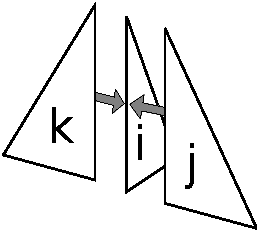
\includegraphics[scale=0.7]{obr7.pdf} 
	\caption{Edge with 3 elements}
	\label{edgemodel}
        \end{center}
      \end{figure}  
  The most general case of connection is relation among $n$ elements like in figure (\ref{edgemodel}). For this case we define
edge element indexset $\mathcal{G}_{l}$ that contains all the indexes of elements which sides make $l$-th edge ($g_l$), so that $\mathcal{G}_{l} = \{i,j,k\}$.
For $\mathcal{G}_{l}$ we introduce its subsets $\mathcal{G}_{ij}$, $\mathcal{G}_{ji}$, $\mathcal{G}_{ik}$, $\mathcal{G}_{ki}$, $\mathcal{G}_{kj}$, and $\mathcal{G}_{jk}$,
  where $\mathcal{G}_{ij} = \mathcal{G}_{ik} =  \mathcal{G}_{l} \backslash {i} = \{j,k\}$, $ \mathcal{G}_{ji} = \mathcal{G}_{jk} = \mathcal{G}_{l} \backslash {j} =\{i,k\}$, and
 $\mathcal{G}_{ki} = \mathcal{G}_{kj} = \mathcal{G}_{l} \backslash {k} =\{i,j\}$. It can be written in the same way for any edge $g$ with more than 3 elements, 
it is hold  $|\mathcal{G}_{g}| - 1 = |\mathcal{G}_{ab}|; \forall a,b \in \mathcal{G}_{g}$.
For $l$-th edge ($g_l$) we can define total edge flow $U_{g_{l}}$ eg. as
  \begin{eqnarray}
   U_{g_{l}} &=& \sum\limits_{m \in \mathcal{G}_{ji}}   \left[ U_{mj}^{+}   + \frac{ U_{jm}^{+}}{|\mathcal{G}_{ji}|} \right] = \sum\limits_{m \in \mathcal{G}_{jk}}  \left[ U_{mj}^{+}   +  \frac{ U_{jm}^{+}}{|\mathcal{G}_{jk}|} \right] \notag \\
	      &=& \sum\limits_{m \in \mathcal{G}_{ij}}  \left[ U_{mi}^{+}   +  \frac{ U_{im}^{+}}{|\mathcal{G}_{ij}|} \right] = \sum\limits_{m \in \mathcal{G}_{ik}} \left[  U_{mi}^{+} +  \frac{ U_{im}^{+}}{|\mathcal{G}_{ik}|} \right] \notag \\ 
	      &=& \sum\limits_{m \in \mathcal{G}_{ki}}  \left[ U_{mk}^{+}   +  \frac{ U_{km}^{+}}{|\mathcal{G}_{ki}|} \right] = \sum\limits_{m \in \mathcal{G}_{kj}}  \left[ U_{mk}^{+}   +  \frac{ U_{km}^{+}}{|\mathcal{G}_{kj}|} \right], \label{edgeflow}
  \end{eqnarray}
$U_{g_{l}}$ with respect to any $e_m$; $m \in \mathcal{G}_{l}$ has to have the same value because continuity equation, for assumed incompresible flow, has to
 be fulfilled in every edge. Edges with more than two elements and two and more nonzero intakes to edge realize an ideal mixing (to an average concentration) 
with weights which will be specified later. This fact modifies equation (\ref{Aeqsol}) on the general mesh into the form
    \begin{equation}
      c_i^{n+1} = c_i^n - \frac{\Delta t}{V_{i}} \left[ \sum_{j \in \mathcal{N}_{i}} \left[ U_{ij}^{+} c_i +  \frac{U_{ij}^{-}}{ \sum\limits_{k \in \mathcal{G}_{ij}}
      \left[ U_{ki}^{+} + \frac{U_{ik}^{+}}{|\mathcal{G}_{ij}|} \right] } \sum\limits_{k \in \mathcal{G}_{ij}} U_{ki}^{+} c_{k} \right] + 
      \sum_{k \in \mathcal{B}_{i}}  \left[  U_{ik}^{e+} c_i +  U_{ik}^{e-} c_{B_{ik}} \right] \right]. \label{Aeqsol2}
    \end{equation}
The edges with total edge flow $U_{g_{l}} = 0$ can occur breakdown in the equation (\ref{Aeqsol2}) via term $\sum\limits_{k \in \mathcal{G}_{ij}}\left[ U_{ki}^{+} + \frac{U_{ik}^{+}}{|\mathcal{G}_{ij}|} \right] = 0$.
This fact implies as well as numerator $U_{ij}^{-} = 0$. In order to avoid dividing by zero we have to assume computation only for nonzero flows.
Concentrations $c_k$, $k \in \mathcal{G}_{ij}$ that may intakes into element $e_i$ are weighted with weights 
\begin{equation}
 \alpha_k = \frac{U_{ki}^{+}}{\sum\limits_{k \in \mathcal{G}_{ij}} \left[ U_{ki}^{+} + \frac{U_{ik}^{+}}{|\mathcal{G}_{ij}|} \right] }, \label{weights}
\end{equation}
so that the ideal mixing in this edge leads to the average concentration 
\begin{equation}
 c_{av} = \frac{\sum\limits_{k \in \mathcal{G}_{ij}} U_{ki}^{+} c_{k}}{\sum\limits_{k \in \mathcal{G}_{ij}} \left[ U_{ki}^{+} + \frac{U_{ik}^{+}}{|\mathcal{G}_{ij}|} \right] }. \label{cav}
\end{equation}
Matrix notation is the same as in (\ref{AeqsolM}). Finally ...

\section{Reaction model}
\input{decay}
\input{semchem}


\end{document}


